\section{美国养老金资产建模}
美国养老金市场资产中的IRA与DC计划部分是积极投资类型的,FOF市场的一大部分投资来源于这两部分养老金资产.所以我们着重研究养老金中IRA与DC计划这两部分资产和的时间序列.由于数据的局限性,我们只搜集到2007-2016年的季度数据,07年之前只搜集到年度数据.
\begin{figure}[h!]
	\begin{minipage}[ht]{0.47\textwidth}
		\centering
		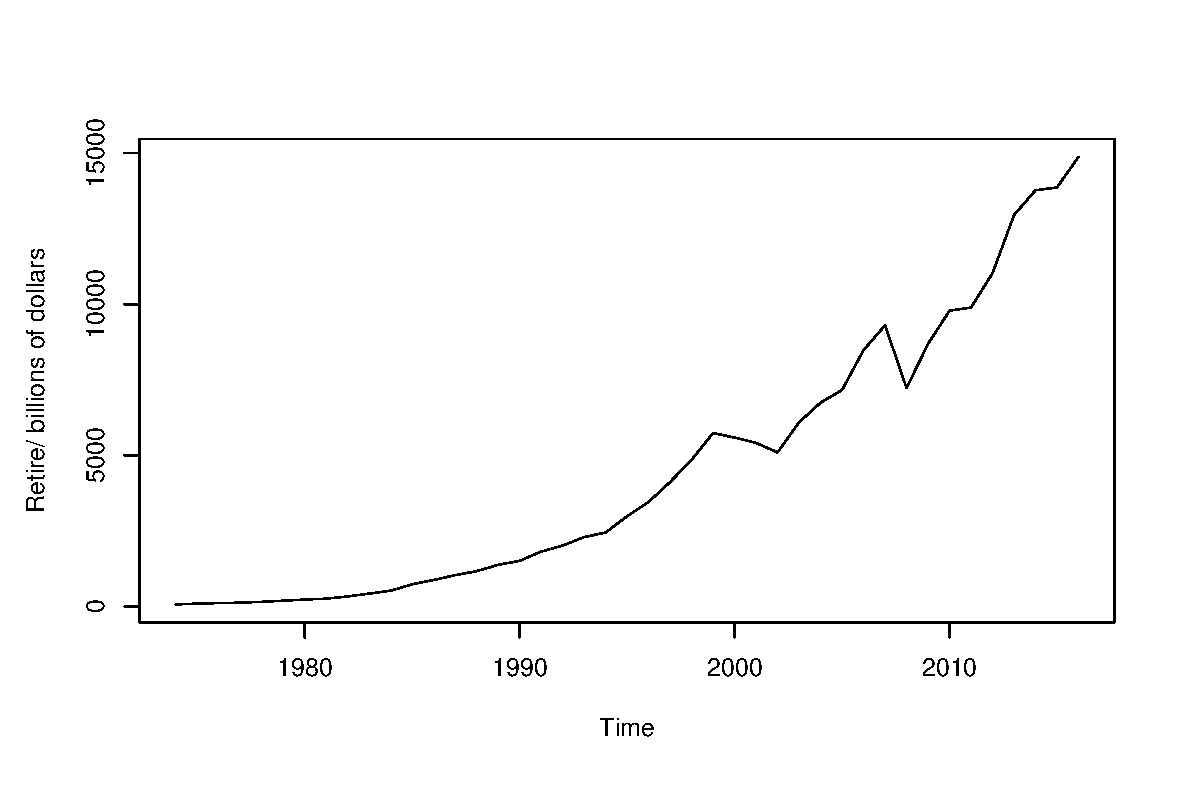
\includegraphics[width=1\textwidth]{pic/re/niandu}
		\subcaption{}\label{niandu}
	\end{minipage}%
	\hspace{0.06\textwidth}
	\begin{minipage}[ht]{0.47\textwidth}
		\centering
		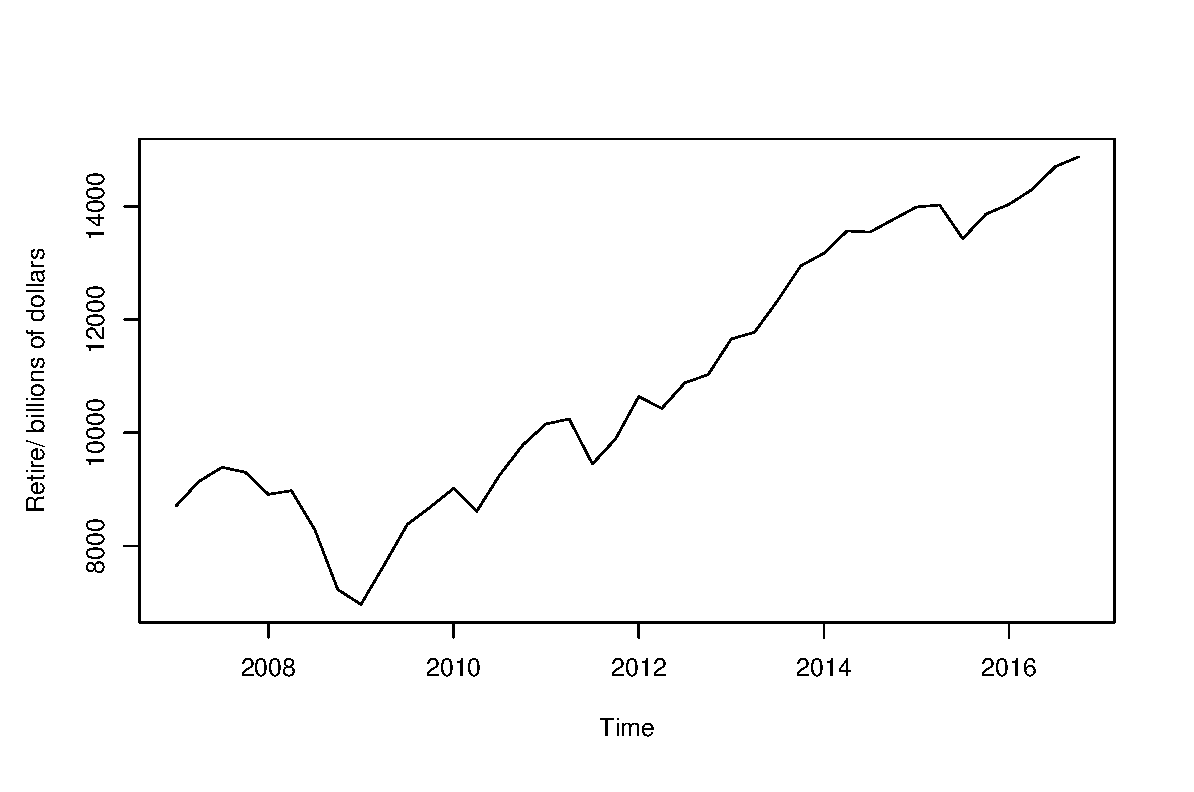
\includegraphics[width=1\textwidth]{pic/re/jidu}
		\subcaption{}\label{jidu}
	\end{minipage}
	\caption{美国养老金资产,IRA+DC部分:(a)1974-2016年IRA+DC年度数据;(b)2007-2016年IRA+DC季度数据}\label{reshuju}
\end{figure}
见图\ref{reshuju},分别是养老金中IRA+DC部分的1974-2016年度数据与2007-2016季度数据.可以看到,序列在2000年之前的波动比较小,在很长一段时间都处于缓慢增长阶段,这与近10年来的情况显著不同,即07年之后的季度数据更具有分析价值.综合考虑,我们采取2007-2016年的季度数据进行建模分析.
\subsection{白噪声序列}
\begin{figure}[h!]
	\centering
	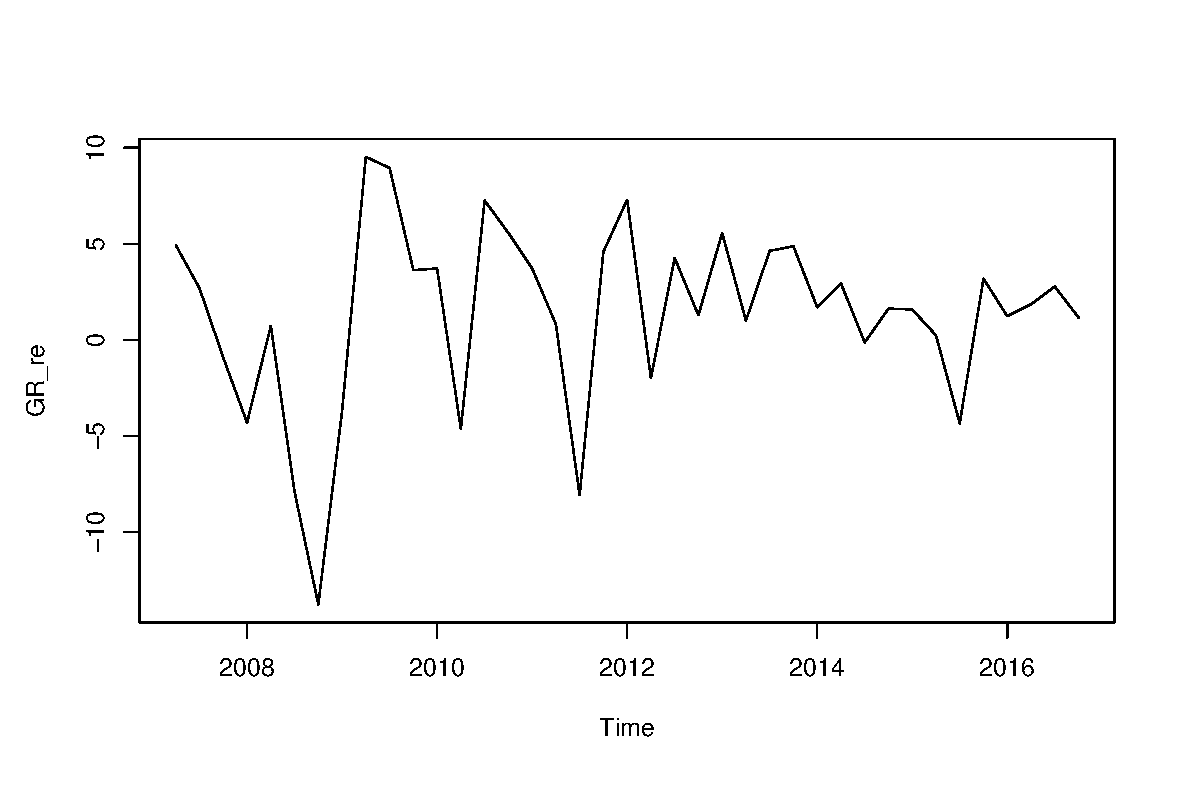
\includegraphics[width=0.5\linewidth]{pic/re/grre}
	\caption{美国养老金资产中IRA+DC部分的对数增长率序列}
	\label{fig:grre}
\end{figure}
如图\ref{fig:grre}所示,我们对上述的养老金季度数据序列进行了对数差分,得到了对数增长率序列.特别的,序列在08年之后出现了相当大的负向波动,这与08年的金融危机对应,由于DC计划可以提前取现,所以在金融危机发生时,发生了较大的资产流失.可以看出,序列大致是平稳的,这一点从ADF检验也可以看到.如下,其$p-value = 0.1231$,在85\%的置信度来说,我们应该拒绝原假设,即序列是平稳的.
\begin{framed}
	\begin{verbatim}
	 	Augmented Dickey-Fuller Test 
	 data:  GR_re
	 Dickey-Fuller = -3.1498, Lag order = 3, p-value = 0.1231
	 alternative hypothesis: stationary
	\end{verbatim}
\end{framed}
进一步,我们对序列进行一阶与二阶Ljung-Box检验,结果如下:
\begin{framed}
	\begin{verbatim}
 	Box-Ljung test                                                   Box-Ljung test
 data:  GR_re                                                       data:  GR_re^2
 X-squared = 14.69, df = 24, p-value = 0.9295              X-squared = 16.588, df = 24, p-value = 0.8657
	\end{verbatim}
\end{framed}
可以看到其一阶与二阶都不存在相关性,即我们可以认为是无异方差的白噪声序列.从McLeod.Li.test也可以看出,见图\ref{fig:mcre},序列不存在ARCH效应.
\begin{figure}[h!]
	\centering
	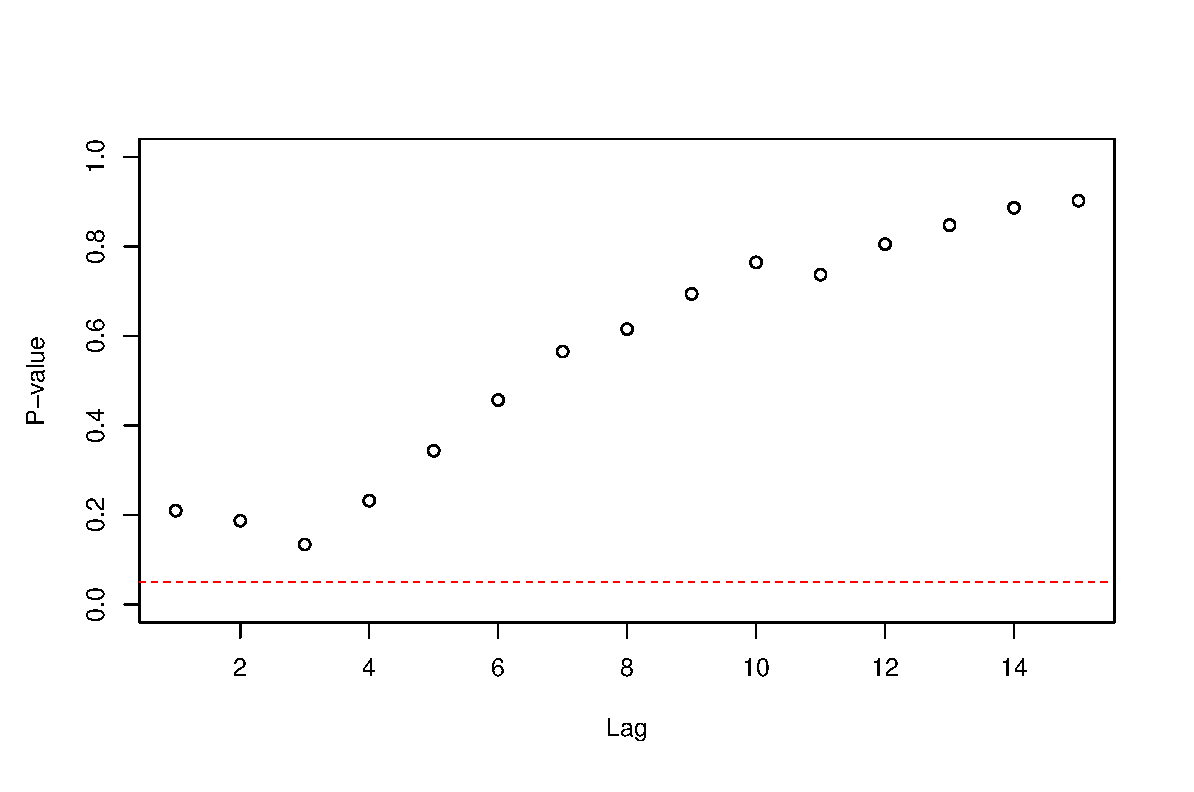
\includegraphics[width=0.5\linewidth]{pic/re/mcre}
	\caption{美国养老金资产中IRA+DC部分的对数增长率序列的McLeod.Li.test检验}
	\label{fig:mcre}
\end{figure}


\subsection{养老金对数增长率序列分布分析}
如前,对养老金对数增长率序列进行分析发现其为近似的白噪声序列,无ARCH效应,故可对该序列的分布进行分析.如图\ref{fig:qqre}所示,
\begin{figure}[h!]
\centering
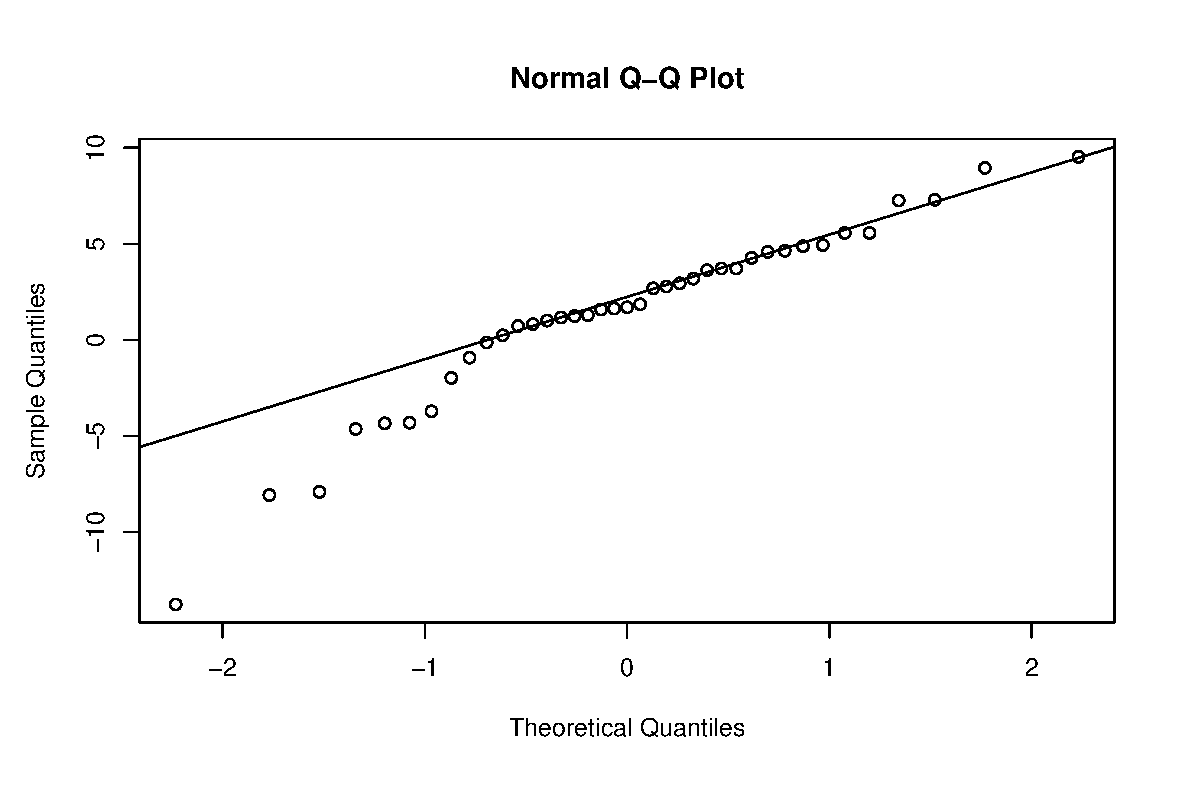
\includegraphics[width=0.5\linewidth]{pic/re/qqre}
\caption{养老金对数增长率序列与正态分布比较的QQ图}
\label{fig:qqre}
\end{figure}
是养老金对数增长率序列与正态分布比较的QQ图,可以看出明显的厚尾分布,并且在负向的厚尾更严重,说明养老金市场资产对负面影响更加敏感.更加具体的还可以从如下的峰度、偏度、Shapiro检验和Jarque Bera检验进行分析.
\begin{framed}
	\begin{verbatim}
	kurtosis(GR_re)                                                   skewness(GR_re)
	1.173374                                                              -0.978918
	\end{verbatim}
\end{framed}
\begin{framed}
	\begin{verbatim}
	Shapiro-Wilk normality test                                           Jarque Bera Test
	data:  GR_re                                                                  data:  GR_re^2
	W = 0.93066, p-value = 0.01887                                   X-squared = 9.9001, df = 2, p-value = 0.007083
	\end{verbatim}
\end{framed}
其中峰度是减去正态峰度后的统计量,可以看到该序列具有一个正的峰度值,即厚尾.由Shapiro-Wilk与Jarque Bera检验也可以看到,都拒绝了原假设,即此序列不是正态分布.

